\section{Ziel}
\label{sec:Ziel}

Die Funktionsweise eines Lock-In-Verstärkers soll kennengelernt und verstanden werden.%Ist das gut so? Irgendwie ein dummes Ziel :D  

\section{Theorie}
\label{sec:Theorie}

Der Lock-In-Verstärker wird genutzt, um bestimmte Eigenschaften einer Signalspannung 
$U_{Sig}$ zu bestimmen. Lock-In-Verstärker werden hauptsächlich zur Messung stark
verrauschter Signale verwendet.

\begin{figure}
    \centering
    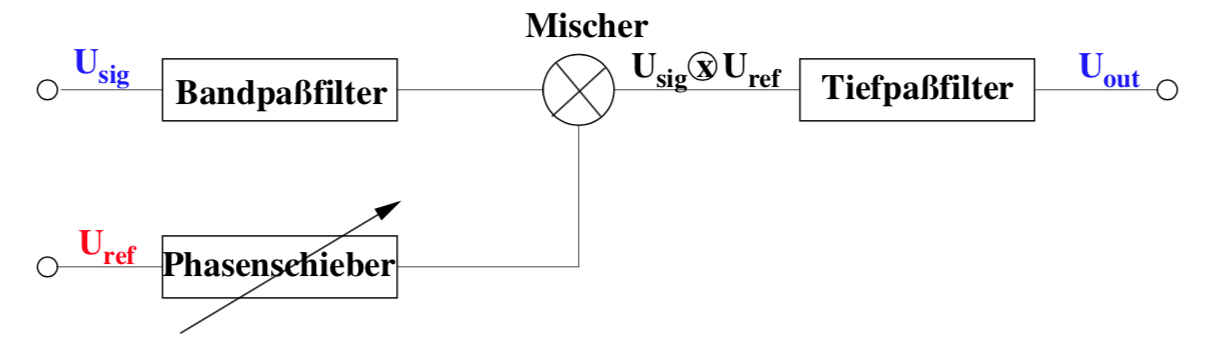
\includegraphics[width=10cm, height=5cm]{build/lockin1.png}
    \caption{Aufbau eines Lock-In-Verstärkers. \cite{V303}}
\end{figure}

\noindent Hierzu wird das das Signal mit einer Referenzfrequenz $\omega_0$ moduliert.
Dieses unter Umständen verrauschte Signal wird durch einen Bandpass von Rauschanteilen 
deutlich höherer oder niedrigerer Frequenzen als der Referenzfrequenz befreit.
In einem sogenannten Mischer wird die Signalspannung $U_{Sig}$ mit einem Referenzsignal 
$U_{Ref}$, das die Referenzfrequenz $\omega_0$ hat, multipliziert. 
% Die Phasenverschiebung zwischen $U_{Sig}$ und $U_{Ref}$ kann durch einen Phasenschieber
% variiert werden.

\noindent Dieses neue Signal wird in einen Tiefpass eingespeist. Dieser hat die 
Eigenschaft, dass er das entstandene Mischsignal über mehrere Perioden der 
Modulationsfrequenz integriert.
Die nicht zur Frequenz synchronisierten Rauschbeiträge werden sich dadurch 
herausmitteln, sodass eine zur Eingangsspannung $U_{Sig}$ proportionale Gleichspannung 
$U_{Out}$ gemessen werden kann. 

\noindent Der Tiefpass entscheidet dabei über die Bandbreite des Restrauschens. 
Je größer die Zeitkonstante des Passes gewählt wird, desto kleiner wird die Bandbreite 
des Rauschens sein. Mit einem Lock-In-Verstärker kann man somit Güten, 
die weit über der Güte eines normalen Bandpasses liegen, erreichen.

\noindent Sind die Signal- und Referenzspannungen nicht in Phase, sondern haben eine 
Phasendifferenz $\varphi$, erhält man die folgende Ausgangsspannung: 
\begin{equation}
    U_{Out} = \frac{2}{\pi}\, U_{0} cos(\varphi).
    \label{eqn:u_out}
\end{equation}
Diese erreicht somit ihr Maximum bei einer Phase von $\varphi = 0$.
Aus der Ausgangsspannung $U_{Out}$ lässt sich die Spannung $U_{0}$ mittels
\begin{equation}
    U_{0} = \frac{U_{Out}\, \pi}{2 cos(\varphi)} %brauchen wir das? sonst weglassen.
    \label{eqn:u_0}
\end{equation}
bestimmen.
